\section{Conception de la solution}

\subsection{Architecture de la solution}

    \subsubsection{Web Service}

    Du coté serveur, il faudra gérer plusieurs parties. D'un coté, il faut s'occuper des requêtes utilisateur, et de l'autre, il faut stocker certaines données que l'on renverra aux utilisateurs.

    Pour ce faire, l'architecture est la suivante.

    \begin{figure}[H]
        \centering
        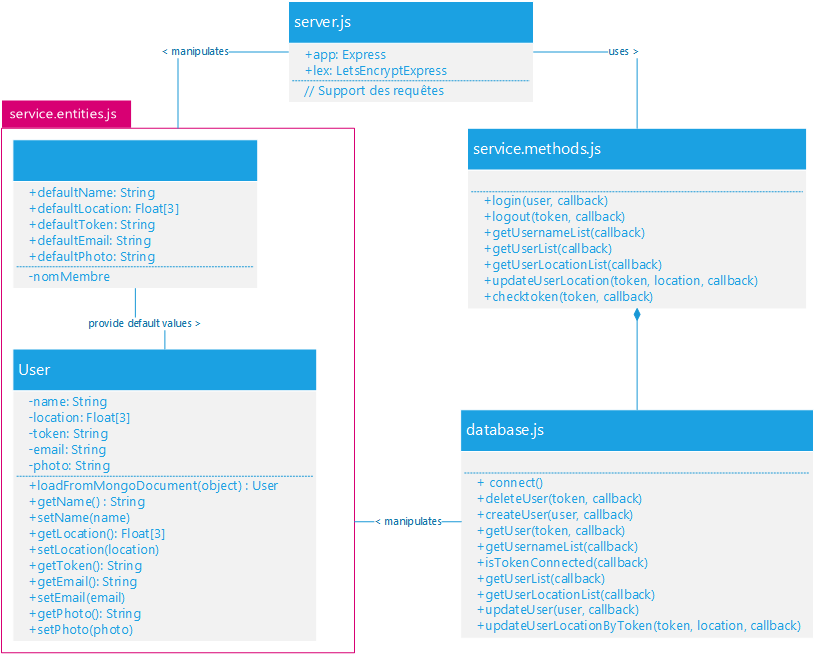
\includegraphics[width=\textwidth]{./img/architecture-service-web.png}
        \caption{Architecture du Service Web}
        \label{asweb}
    \end{figure}

    Comme nous pouvons l'observer dans la figure \ref{asweb}, blablabla.
    Le serveur + Mongodb.
    Pattern bridge pour la bdd. Des entités.

    \subsubsection{Application Android}

Le développement du client mobile a suivi le schéma classique de conception d’une application Android. Pour rappel les objectifs initiaux majeurs de ce client étaient de pouvoir récupérer des données sur un web service, les exploiter, les afficher à l’utilisateur et enfin retourner des données au service en question. De façon général la solution Android s’organise en deux projets directeurs : les tests et l’implémentation de l’application.

Il n’a pas été choisi ici de faire du développement dirigé par les tests car la technologie Android était dans le cadre de ce projet une découverte et il aurait était hasardeux de définir des tests Java sur les concepts Android. Les tests ont donc ici vocation à valider les mécaniques métiers a posteriori ainsi que le bon fonctionnement et l’intégrité de l’application au fur et à mesure de l’ajout de fonctionnalités. La partie relative aux tests se subdivise en deux autres : les tests unitaires et les tests instrumentés. Les premiers sont plutôt classiques et permettent de tester les mécaniques métiers et de vérifier tout ce qui est mockable, autrement dit simulable. Toutefois, il y a certains aspects dans un programme Android qu’il n’est pas possible de mocker sans enlever l’intérêt du test. Nous parlons ici de fonctionnalités s’appuyant intrinsèquement sur le système Android comme les appels réseaux, le GPS, l’écran, etc. Il est nécessaire dès lors que l’on veut simuler une fonctionnalité Android même basique, de simuler tout un système Android. D’où l’intérêt de la deuxième catégorie de tests : les tests instrumentés. Ceux-ci vont être exécutés sur un émulateur Android directement afin de pouvoir tester dans notre cas les appels réseaux et l’utilisation du GPS.

Le projet de tests est donc un projet annexe venant en soutien au projet principal : celui du développement de l’application Android. L’ensemble doit gérer des données et les afficher, c’est pourquoi un modèle MVC semblait adapté. Le modèle MVC se compose de trois parties en interaction comme c’est visible figure \ref{mvc}.

\begin{figure}[H]
    \centering
    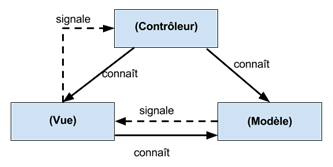
\includegraphics[width=\textwidth]{./img/mvc.png}
    \caption{Patron de conception MVC}
    \label{mvc}
\end{figure}

Le modèle (M) représente les données traitées, dans le cas de l’application ce sont principalement les utilisateurs et leur position GPS. Les deux autres composants n’interagissent pas directement avec les données brutes mais ont accès à l’\underline{API} du modèle symbolisée par le gestionnaire d’utilisateur (UserManager) comme sur la figure \ref{model}. Le modèle gère donc tous les petits traitements bas niveau sur les données et les sert au reste de l’architecture selon les besoins.

\begin{figure}[H]
    \centering
    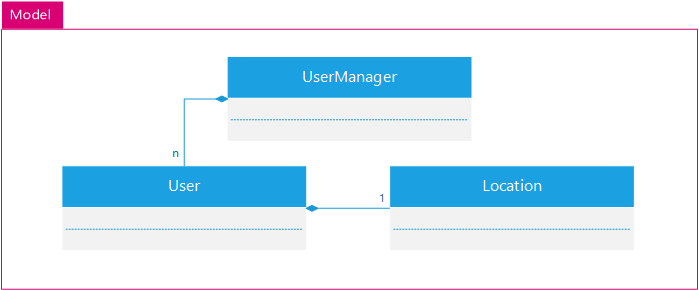
\includegraphics[width=\textwidth]{./img/android-model.png}
    \caption{Diagramme du modèle}
    \label{model}
\end{figure}

Le contrôleur (C) s’occupe des interactions avec l’utilisateur, il doit pouvoir transmettre les commandes émanant de l’utilisateur aux autres composants. Dans le cadre de l’application Android, le contrôleur est symbolisé par les \underline{activités} : ce sont les activités Android qui proposent les interfaces de contrôle utilisateur. Elles permettent de recevoir les évènements utilisateur comme un clic ou encore les messages du système comme l’arrivée d’un SMS ou encore l’actualisation de la position GPS. Les informations reçues peuvent ensuite être utilisées pour effectuer une mise à jour du modèle ou un rafraîchissement de l’affichage. Les différents types d’activités sont visible sur la figure \ref{controller}.

\begin{figure}[H]
    \centering
    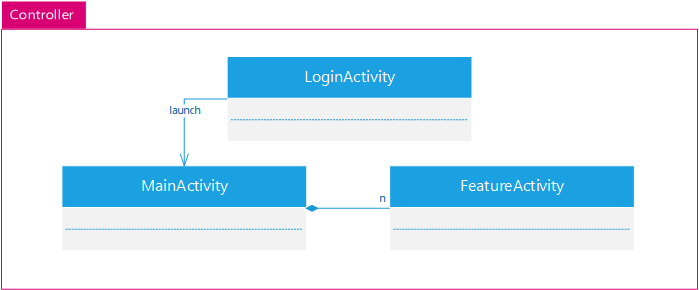
\includegraphics[width=\textwidth]{./img/android-controller.png}
    \caption{Diagramme du contrôleur}
    \label{controller}
\end{figure}


La vue (V) est l’ensemble des éléments constituant la façon dont vont être présentées les données. La réalisation concrète dans l’application Android de la vue est faite par les fichiers XML de layout et autres ressources. Dans la vue entre aussi un pan important du concept de l’application : la gestion de l’affichage 3D. En effet, pour la plupart des éléments d’interface, tout peut être géré par des fichiers de métadonnées mais pour générer la carte en trois dimensions d’un lieu il est nécessaire de décrire dans le code la manière d’utiliser les données pour les afficher avec de véritables classes Java. La vue est donc un ensemble complexe constitué de diverses ressources comme on peut le voir sur la figure \ref{view}.

\begin{figure}[H]
    \centering
    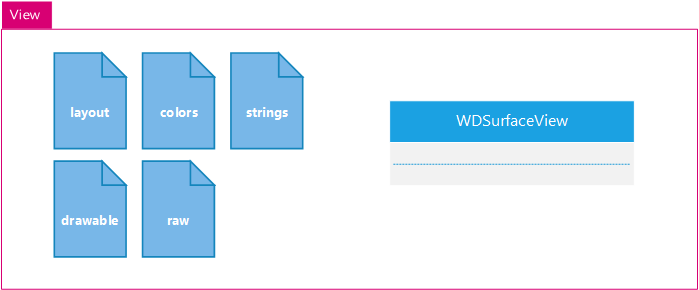
\includegraphics[width=\textwidth]{./img/android-view.png}
    \caption{Diagramme de la vue}
    \label{view}
\end{figure}

Le tout s’interconnecte et interagit donc pour faire fonctionner l’ensemble. Mais pour alimenter l’application en données exploitables, des services ont dû être mis en place. Il en existe deux qui servent de sources de données au programme. Le premier est le service GPS, il permet à l’application de récupérer la position du dispositif Android. Dans un premier temps, ce service été basé uniquement sur les données matérielles de l’appareil mais afin d’améliorer la précision, l’utilisation des Google Services a été choisie. Les Google Services utilisent à la fois les données GPS pures mais aussi leur historique ainsi que les données du gyroscope et de l’accéléromètre pour déterminer la position avec une plus grande précision. Ceci s’est avéré indispensable pour une localisation correcte en intérieur.

Le deuxième service est celui responsable de la communication avec le serveur et qui permet de le requêter. Ainsi ce service permet à la fois d’envoyer sa propre position au serveur mais aussi de récupérer la liste des utilisateurs connectés et leurs informations. Ce service exécute en parallèle du thread principal des requêtes http sur le web service WatchDogZZ. Pour ce faire, il utilise la bibliothèque Volley qui permet d’effectuer simplement des communications sur le réseau.

Le patron de conception majeur dans ce système applicatif est celui observer-observable : il permet à une des entités d’être prévenue par une autre après inscription qu’un traitement a été effectué. Ceci permet le parallélisme des services et de ne pas bloquer l’interface graphique lors d’un traitement long (communication réseau).

L’ensemble est sécurisé par le système d’authentification Google. Ce choix a été motivé par la simplicité puisque le client étant sur un système Android, il possède forcément un compte Google associé. Il suffit alors d’effectuer une requête sur les serveurs de Google avec les informations d’authentification de l’appareil pour récupérer un token validant l’identité de l’utilisateur. Ce token est ensuite transmis lors de chaque requête au serveur WatchDogZZ en vue de vérifier l’identité du demandeur (voir la figure \ref{token}).

\begin{figure}[H]
    \centering
    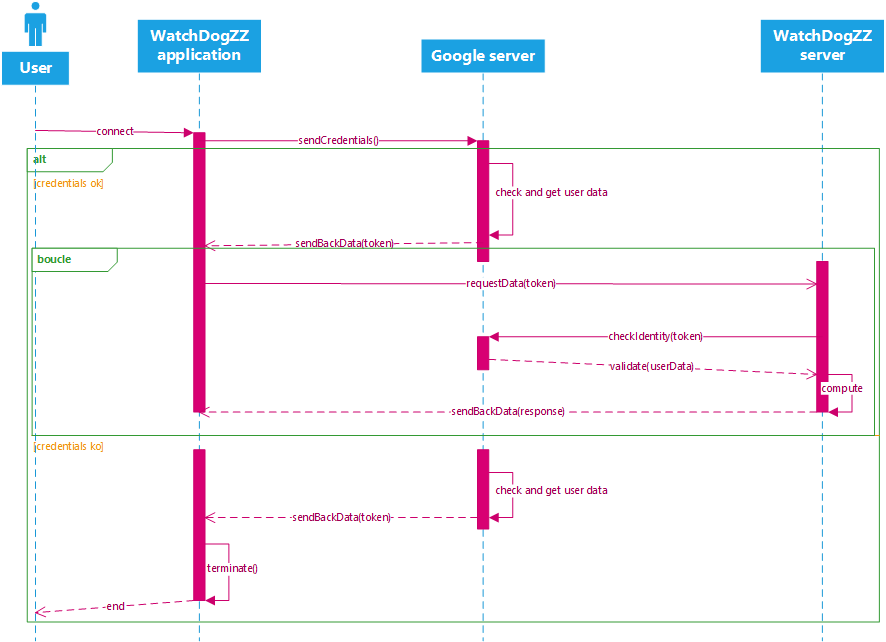
\includegraphics[width=\textwidth]{./img/android-token.png}
    \caption{Utilisation du token Google}
    \label{token}
\end{figure}

La carte du maraudeur est une vue qui a été créée spécialement pour l’application. Elle se base sur une SurfaceView reposant sur de l’OpenGL ES 2. L’intérêt était à la fois de pouvoir dessiner en deux mais aussi trois dimensions. Un Renderer spécial a été implémenté ainsi que des managers de ressources 3D. Il est ainsi possible de gérer cette vue comme un observer du UserManager. La vue pourra par la suite afficher les scènes 3D avec les différents éléments à chaque notification. Les différentes classes entrant en jeu sont visibles sur la figure \ref{3d} ainsi que leur rôle dans le MVC.

\begin{figure}[H]
    \centering
    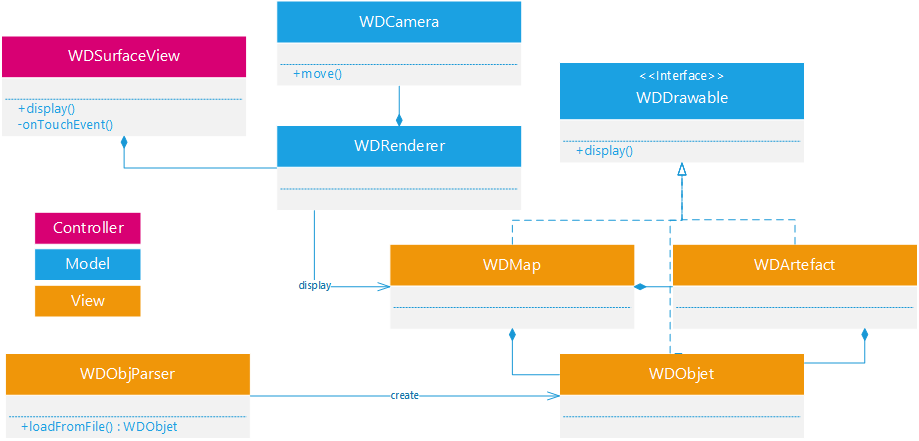
\includegraphics[width=\textwidth]{./img/android-3d.png}
    \caption{Fonctionnement de la 3D Android}
    \label{3d}
\end{figure}

La conception de l’application Android est très simple mais fait intervenir de nombreux éléments et services qui touchent énormément d’aspects de la programmation Android. Il existe sur les versions les plus récentes du Framework des fonctionnalités plus intéressantes et performantes toutefois le choix a été fait d’essayer de faire l’application la plus diffusable possible et donc de supporter un maximum d’appareil. Au début du développement, la version choisie était la 9 mais suite à des contraintes inévitables de développement nous avons dû monter à la version 12. Ceci reste correct d’autant plus que cela représente toujours plus de 99\% du marché Android.

\subsection{Technologies utilisées}

    \subsubsection{Service Web}

Pour la conception du Service Web, nous avions besoin d'une technologie disposant des caractéristiques suivantes :
\begin{itemize}
    \item Facile à utiliser ;
    \item Disposant de nombreuses fonctionnalités ;
    \item Rapide à l'exécution ;
    \item Exécution légère sur serveur ;
    \item Configuration rapide.
\end{itemize}

Toutes ces caractéristiques se retrouvent avec le framework NodeJS \cite{nodejs}. C'est un framework Javascript qui dispose de nombreuses librairies installables à l'aide du gestionnaire de modules NPM \cite{npmjs}. De plus, étant donné que l'un d'entre-nous avait déjà utilisé une telle technologie, cela nous permettait de démarrer plus rapidement.

Le gestionnaire de modules NPM permet d'effectuer plusieurs choses.
Premièrement c'est lui qui va permettre l'installation des modules nécéssaires au bon fonctionnement du Service. Ensuite, il va se charger de résoudre les dépendances entre modules. C'est à dire que si un module à besoin d'un autre module pour fonctionner, alors celui-ci sera installé automatiquement.
Enfin, il est possible de disposer de plusieurs listes de modules à installer :
\begin{description}
    \item [Production] : comporte les modules nécéssaires au lancement du Service en mode production, donc sans les outils de debug ;
    \item [Dev] : comporte les modules installés en production ainsi que des modules complémentaires utilisés lors de la conception du Service ou à des fins de debuggage.
\end{description}

Afin de mettre en place notre Service Web, nous avons utilisés plusieurs modules :
\begin{description}
    \item [Body-parser] : parser le contenu JSON des requêtes ;
    \item [Express] : créer un serveur Http ou Https ;
    \item [Jasmine] : effectuer des tests de spécifications ;
    \item [Letsencrypt-express] : gérer les certificats Https du serveur ;
    \item [Mongodb] : système de gestion de base de données ;
    \item [Request] : effectuer des requêtes http ou https ;
    \item [Winston] : faire des logs sur plusieurs niveaux (info, error, warning, debug).
\end{description}

    \subsubsection{Android}

Le développement d'une application Android s'effectue généralement en utilisant le Java ainsi qu'Android Studio \cite{androidstudio}, permettant d'inclure les bibliothèques Android. Ici, nous avons donc utilisé ces technologies pour permettre une intégration parfaite sur les systèmes Android.

Android est un système d’exploitation à destination des plateformes mobiles supporté par Google et basé sur un noyau Linux. Il équipe aujourd’hui plus de 80\% des terminaux mobiles mais s’adapte aussi sur une large gamme de produits : smartphones, tablettes, montres, téléviseurs, etc. Les systèmes Android sont capables d’exécuter des programmes dérivés du Java grâce à leur environnement d’exécution : une machine virtuelle Dalvik ou l’Android Runtime selon la version. Il est donc possible de produire des exécutables de type apk à base de Java en s’appuyant sur le \underline{SDK} Android, à la rédaction de ce rapport l’API la plus récente est la 25.

La programmation Android est donc très proche du développement d’applications Java modernes mais comporte tout de même des concepts spécifiques apportées par le SDK. On peut citer par exemple le concept d’activité qui représente une vue dans une application ou encore un intent qui est une demande de service qu’une application peut envoyer au système. L’API propose aussi une pléthore de fonctionnalités utilisant les composants du terminal mobile : gps, accéléromètre, appels réseaux, contacts, sms, etc.

En plus du SDK Android, notre projet nécessite l’utilisation de trois autres bibliothèques : les Google Services, Volley et OpenGL ES. 

Le premier, les Google Services, est un ensemble de fonctionnalités avancées fournies par Google. Les Google Services permettent à tous ceux utilisant un terminal Android d’accéder aux dernières fonctionnalités sans pour autant avoir la dernière version de l’OS. La subtilité derrière ces services est qu’officiellement, Android est censé être un système open source, toutefois pour garder la maitrise du produit Google a décidé de freiner sa participation au cœur d’Android et propose ses meilleurs services et évolutions au travers des Google Services ce qui leur permet de rendre Android presque totalement dépendant de Google. Le géant américain participe donc de façon fermée à un projet open source en empêchant toute concurrence. Dans le cadre de ce projet c’est le système de géolocalisation amélioré qui nous intéresse dans ces services. En effet, la version Android fourni juste la position donnée par le capteur alors que les Google Services prennent en compte plusieurs paramètres comme l’historique de position, les mouvements, les déplacements, etc.

La bibliothèque Volley permet d’effectuer des requêtes réseaux avec une plus grande facilité. Comme on peut le voir sur la figure \ref{volley}, Volley est capable d’exécuter des appels asynchrones et de cacher les réponses. Les gains en performances et en expérience utilisateur sont donc tout à fait de la partie.

\begin{figure}[H]
    \centering
    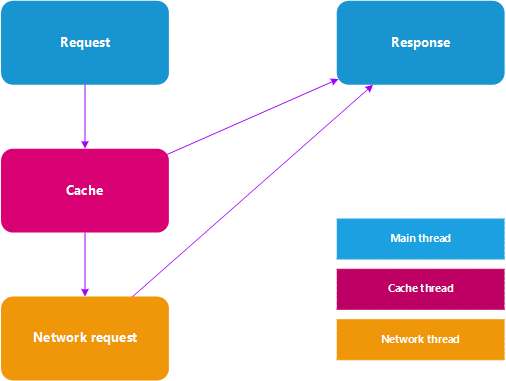
\includegraphics[height=8cm]{./img/volley.png}
    \caption{Fonctionnement d’un requête Volley}
    \label{volley}
\end{figure}

Cette bibliothèque apporte donc des fonctionnalités d’un peu plus haut niveau que le basic HttpUrlConnection de java.net si l’on considère les appels implicites à d’autres threads et des performances améliorées grâce au caching (pour le chargement d’images par exemple).

Enfin le dernier framework utilisé est OpenGL ES ou Embedded System. Ce n’est autre que la version portable du célèbre framework graphique qui a été conçu spécialement pour la programmation embarquée. Comme son ainée, cette version dispose d’une API de bas niveau mais permet au moins de réaliser énormément de choses. En effet il aurait été possible d’utiliser le framework Unity (haut niveau) comme beaucoup d’applications 3D le font, mais cela implique d’utilise des ressources propriétaires payantes alors que les vues 3D à développer dans notre cas ne sont pas très évoluées.

La dernière technologie à présenter en lien direct avec Android est bien sûr l’\underline{IDE} utilisé. Nous avons opté pour Android Studio, visible sur la figure \ref{androidstudio}, qui est l’environnement de développement officiel d’Android. Android Studio s’inspire grandement des autres outils de la société JetBrains en intégrant beaucoup d’utilitaires spécifiques au développement Android. Il existe d’autres solution comme des versions ou même des plugins Eclipse mais depuis l’arrivée en 2014 d’Android Studio, il n’est vraiment pas recommandé d’utiliser encore Eclipse. Un autre, Processing permet d’effectuer du développement Android mais on est quand même loin de l’outil de JetBrains au niveau des fonctionnalités.

\begin{figure}[H]
    \centering
    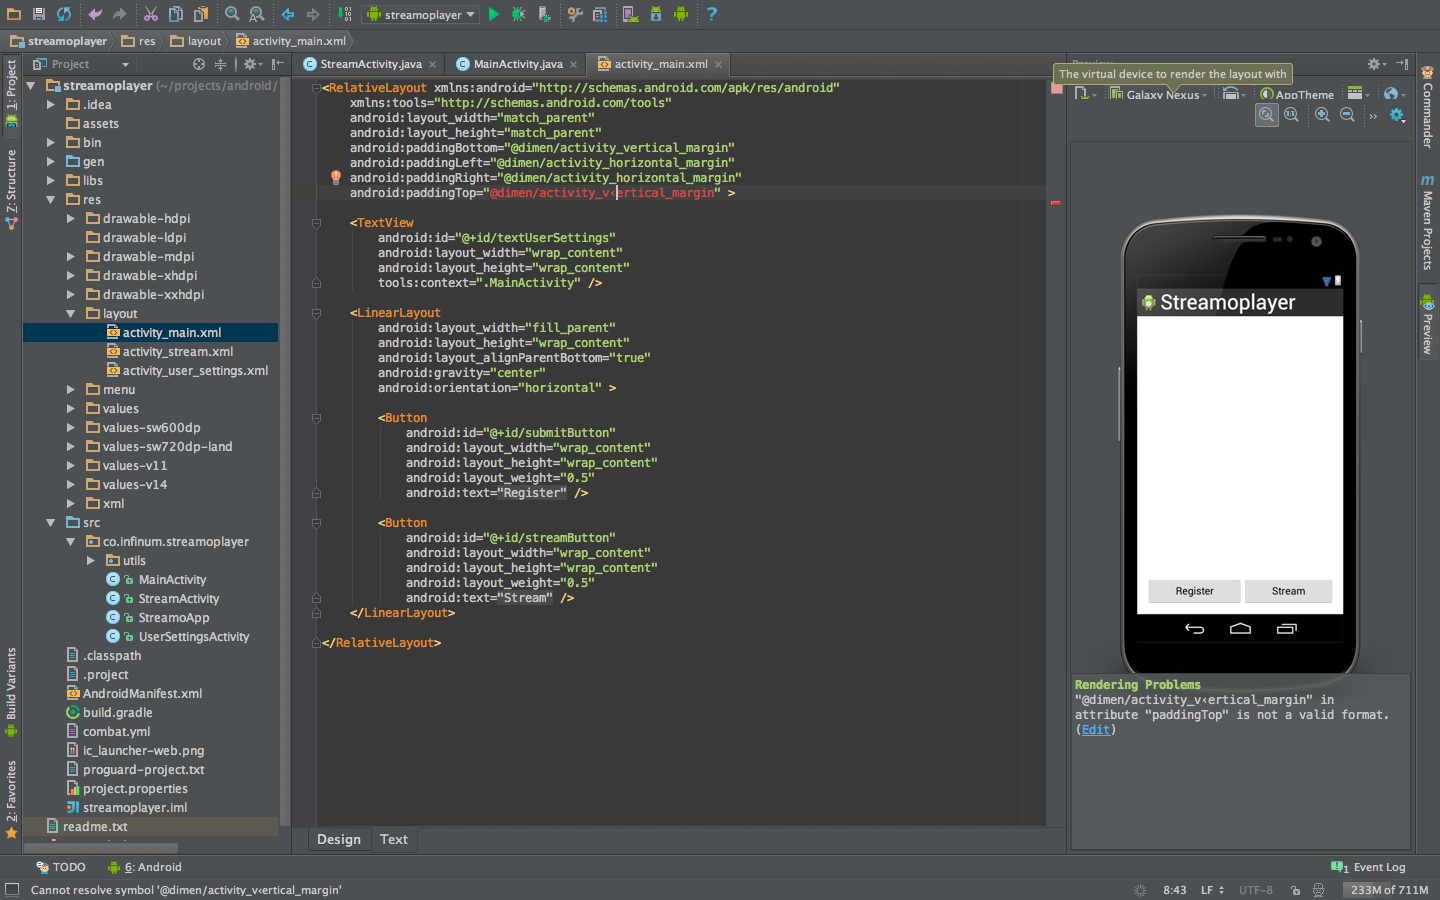
\includegraphics[width=\textwidth]{./img/android-studio.png}
    \caption{Environnement de développement intégré officiel d’Android}
    \label{androidstudio}
\end{figure}

Nous n’allons pas passer en revue ici toutes les fonctionnalités d’Android Studio qui comporte bien sûr toutes les fonctionnalités que l’on peut attendre d’un environnement professionnel mais il faut remarquer qu’il dispose d’outils remarquables.

Le premier est son gestionnaire de SDK : celui-ci permet de maintenir à jour et de manipuler toutes les versions de SDK disponibles. C’est plutôt utile pour un développement où chaque client est différent même si cela reste de l’Android.

Le second est la mise à disposition d’émulateurs Android. Il permet de simuler des terminaux Android de toutes sortes sans besoin de disposer du matériel en réalité. De plus le moniteur intégré permet de suivre en détail l’activité du simili-système ce qui est un plus lors de l’analyse d’exécution d’une application.

Enfin, Android Studio permet de développer les interfaces graphiques soit en mode texte soit en mode \underline{WYSIWYG} ce qui peut avoir l’avantage d’avoir une prévisualisation d’une vue sans avoir à exécuter toute l’application.

Nous allons maintenant aborder les technologies tierces utilisées au cours de ce projet.

\subsection{Fonctionnalités introduites}

    Dans cette partie, nous allons traiter des différentes fonctionnalités présentées par la solution. Nous aborderons tant le point de vue des applications utilisatrices de ce service, que le point de vue de la gestion du service.

\subsubsection{Concepts introduits}

Avant de présenter les diverses fonctionnalités, certains mécanismes visant à la qualité du service vont être présentés.

Pour commencer, un service de \underline{DNS} est utilisé. Ce type de service permet d'attribuer une URL textuelle à un adresse IP (l'adresse du serveur web). Ainsi, les utilisateurs retiendront plus facilement cette URL plutôt que l'adresse IP, et cela permet de configurer les applications clientes plus facilement (en renseignant simplement l'URL textuelle).

De plus, il faut noter que dans certains cas, l'adresse IP d'un serveur n'est pas attribuée de manière statique. Pour remédier à cela, nous avons ajouté un service \underline{DynDNS}. Ce service va mettre en place un mécanisme mettant à jour l'adresse IP à associer à l'URL textuelle définie avec le DNS. De ce fait, il n'y a plus besoin de s'occuper des changements dynamiques d'IP du serveur web. Grâce à cela, nous pourrons toujours accéder au service à l'aide de l'URL \textbf{https://watchdogzz.ddns.net}.

Comme nous pouvons le constater dans l'URL fournie précédement, nous utilisons le protocole \textbf{\underline{https}}. Comme l'indique son dernier 's', celui est est sécurisé par une couche de chiffrement \underline{TLS}. Cette couche de chiffrement va s'occuper de \underline{chiffrer} les données fournies dans la requête de l'utilisateur, qui ne seront donc pas visible si une personne parvient à intercepter la requête.
Pour introduire ce concept, le paquet \textbf{Letsencrypt-express} est utilisé et vient compléter le serveur \textbf{Express}. Ce paquet va en fait utiliser le service en ligne Letsencrypt~\cite{letsencrypt}, qui va se charger de gérer automatiquement les certificats relatifs à l'authentification du serveur ainsi que l'envoie des informations d'authentification et de chiffrement au client. Ce service permet donc de disposer d'une autorité de certification valide, et donc d'assurer aux utilisateurs que ce service est bien celui qu'ils demandent, et non un service malicieux.

Un dernier mécanisme introduit dans le service est celui du \textbf{logger}. Ce mécanisme consiste à enregistrer dans des fichiers (généralement dits "de log") certaines actions qui s'effectuent sur le service. Nous pouvons par exemple décider d'enregistrer des informations de contrôle relative au démarrage du service, des erreurs système, ou encore des informations de \underline{debug} lors de l'ajout de nouvelles fonctionnalités.

Ce qui va nous intérésser principalement avec le logger, c'est la possibilité de pouvoir analyser les requêtes renvoyant des erreurs aux utilisateurs.
De ce fait, si nous sauvegardons suffisament d'informations lorsqu'une requête échoue, nous serons capable de déterminer la cause de l'erreur, et ainsi éventuellement corriger un comportement menant à des erreurs involontaires.

Le logger est mis en place à l'aide du module \textbf{Winston}, et va permettre de gérer les fichiers de log suivants :
\begin{itemize}
    \item \textbf{server-error.log} : erreurs critiques du serveur, de la base de données erreurs de requêtes ;
    \item \textbf{server-info.log} : informations de contrôle sur le serveur ;
    \item \textbf{server-debug.log} : informations utilisées lors du développement de nouvelles fonctionnalités.
\end{itemize}

Il faut noter que lorsque l'on souhaite logger une information (normale ou une erreur), il faut indiquer son niveau de sévérité. Avec le module ici utilisé, les niveaux sont les suivants (un niveau plus bas implique une importance plus grande) :
\begin{enumerate}
    \item \textbf{Error}
    \item Warn
    \item \textbf{Info}
    \item Verbose
    \item \textbf{Debug}
    \item Silly
\end{enumerate}

Les fichiers de log décrits précédement correspondent chacun à un niveau de sévérité. Ainsi, nous aurons dans le fichier \textbf{server-error.log} uniquement les erreurs, ce qui permet un traitement facile de celles-ci ; dans le fichier \textbf{server-info.log}, nous disposerons d'informations de contrôle et des erreurs ; et enfin dans le fichier \textbf{server-debug.log}, nous disposerons des erreurs, informations de contrôle et informations de debug.

\subsubsection{Utilisation du service}

La principale fonctionnalités du Service Web est de répondre à des requêtes. Des URL sont mises à disposition par le service et permettent d'effectuer certaines tâches. Le passage de paramètres pour ces URL se fait directement dans le corps de la requête sous forme de JSON.
Les réponses du service sont également sous forme d'objet JSON dans le corps de la réponse.
Le paquet \textbf{Body-parser} utilisé dans le serveur permet d'effectuer le parsing automatique du corps de la requête pour le transformer en JSON, utilisable dans le code.

En cas d'erreurs, les réponses contiennent les champs suivants :
\lstset{language=Javascript}
\begin{lstlisting}[caption=Corps général de la réponse serveur]
{
    'status': 'ok' / 'fail', // L'état de la requête
    'error': 'description' // Une description de l'erreur s'il y en a une, sinon ce champ est absent
}
\end{lstlisting}

La plupart des requêtes décrites nécéssitent que l'utilisateur soit authentifié. Pour ce faire, il doit effectuer une première requête sur l'URL \textbf{/login} en utilisant la méthode \textbf{POST}. Les paramètres suivants sont attendus par le service :
\lstset{language=Javascript}
\begin{lstlisting}[caption=Corps de la requête POST /login, label=postlogin]
{
    'name': 'username', // Le nom de l'utilisateur à connecter
    'token': 'azertyuiop12345', // Le token de connexion fourni par Google
    'location': [1.0, 2.0, 3.0], // La position courrante de l'utilisateur
    'photo': 'http://photo/user1', // L'URL vers la photo de l'utilisateur
    'email': 'mail@example.com' // L'adresse mail de l'utilisateur
}
\end{lstlisting}

Notons que les champs \textbf{photo} et \textbf{email} sont optionnels. S'ils ne sont pas renseignés lors de la connexion, des données par défaut seront utilisées. Ce données pourraient par exemple venir à manquer si l'utilisateur ne souhaite pas donner son adresse mail, ou si par exemple il ne possède pas de photo (auquel cas une photo par défaut doit effectivement être utilisée par le client).

Le service est capable de retourner la liste des personnes connectée sur le Service en effectuant une requête de type \textbf{GET} sur l'URL \textbf{/who}. Le résultat est transmis sous la forme suivante :
\lstset{language=Javascript}
\begin{lstlisting}[caption=Corps de la réponse GET /who]
{
    'list': [
        'userName1',
        'userName2',
        'userName3'
    ]
}
\end{lstlisting}

Si l'on souhaite disposer d'informations supplémentaires en plus du nom des personnes connectées (url de photo, position, adresse mail), il est possible d'effectuer une requête \textbf{GET} sur l'URL \textbf{/where}.
\lstset{language=Javascript}
\begin{lstlisting}[caption=Corps de la réponse GET /where]
{
    'list': [
        {
            'name': 'username1',
            'location': [1.0, 2.0, 3.0],
            'photo': 'http://photo/user1',
            'email': 'mail1@example.com'
        },
        {
            'name': 'username2',
            'location': [4.0, 5.0, 6.0],
            'photo': 'http://photo/user2',
            'email': 'mail2@example.com'
        },
        {
            'name': 'username3',
            'location': [7.0, 8.0, 9.0],
            'photo': 'http://photo/user2',
            'email': 'mail3@example.com'
        }
    ]
}
\end{lstlisting}

Pour mettre à jour sa position sur le Service, l'utilisateur effectue une requête sur cette même URL \textbf{/where}, mais cette fois avec la méthode \textbf{POST}, et en spécifiant les champs suivants dans le corps de sa requête :
\lstset{language=Javascript}
\begin{lstlisting}[caption=Corps de la requête POST /where]
{
    'token': '1A2Z3E4R5T6Y7U8I9O0P',
    'location': [1.0, 2.0, 3.0]
}
\end{lstlisting}

Cette requête peut également permettre de connecter un utilisateur directement si celui-ci ne l'est pas déjà. En effet, puisque son token de connexion est fourni (et peut permettre de l'identifier de manière unique), il est possible de vérifier s'il est connecté (auquel cas, sa position est mise à jour simplement), sinon, nous allons pouvoir le connecter en utilisant les informations qu'in va nous fournir. Il est possible de fournir les mêmes informations que dans le code~\ref{postlogin}. Ainsi l'utilisateur sera créé avec les informations qu'il a soumises et sa position initiale est enregistrée. Il peut ensuite effectuer de simples requêtes POST sur l'URL /where pour mettre à jour sa position.

Ces requêtes, lorsque effectuées correctement sur le service, ne retournent pas d'erreurs. Cependant, il est possible que dans certains cas, elles n'aient pas fonctionnées sur le serveur, pour plusieurs raisons :
\begin{itemize}
    \item Le service connaît une erreur interne (configuration, crash) ;
    \item Le service ne parvient pas à communiquer avec la base de données ;
    \item La requête utilisateur ne fourni pas les informations suffisantes au traitement de sa requête.
\end{itemize}

Pour indiquer cela à l'utilisateur, le code de retour de la requête est choisi parmis les suivants :
\begin{itemize}
    \item Pas d'erreur : code 200 ;
    \item Erreur interne ou paramètres insuffisants pour la requête : erreur 400 ;
    \item Erreur de communication avec la base de données : erreur 503.
\end{itemize}

Ces erreurs peuvent par la suite être gérées par le client. Il peut ainsi choisir soit de réitérer sa requête (dans le cas d'une erreur 503 par exemple), soit d'informer l'utilisateur que le service est indisponible ou que sa requête n'est pas valable (cas d'une erreur 400).

Le diagramme suivant (figure~\ref{servicereq}) permet de mieux apprécier l'enchaînement des requêtes ainsi que leur cheminement sur le serveur. Pour des raisons de simplification, nous représenterons l'utilisateur comme une application capable d'utiliser correctement le service ainsi que toutes ses fonctionnalités.

\begin{figure}[H]
    \centering
    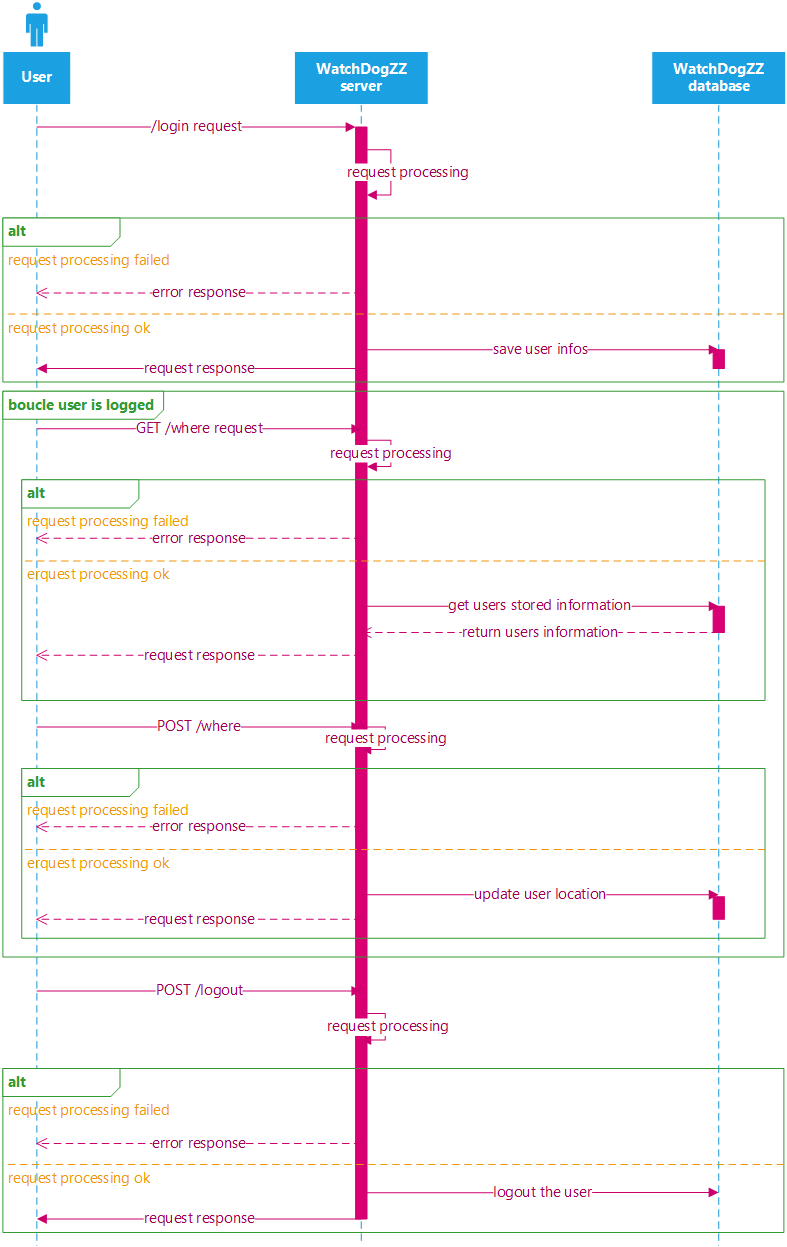
\includegraphics[height=0.99\textheight]{./img/server-requests.png}
    \caption{Diagramme de séquence des requêtes sur le service}
    \label{servicereq}
\end{figure}

    
    \input{./part/fonc-android}

\subsection{Méthodes de développement}

La méthode adoptée pour la conception de cette solution devait pouvoir convenir à un projet hétérogène et à une équipe de taille faible, un binôme. De façon générale le projet se décomposait en trois sous-projets indépendants : la partie serveur, la partie client et la partie documentation.

La partie documentation est la seule qui a réellement fait l’objet d’un travail commun avec concertation, échange de points de vue et vérification du travail de l’autre puisqu’elle a consisté en la mise au point des spécifications et en la rédaction de ce rapport. Durant la phase d’analyse et devant l’état des lieux de tout ce qui devait être fait, il a paru équitable et logique de détaché une personne sur le projet Android et une autre sur le projet serveur. Ainsi la répartition des tâches et l’expertise sur les différents projets étaient très contrôlé.

Une fois que les besoins de l’application ont été analysés et que les spécifications ont été posées, nous avons transformé ses documents en un kanban regroupant les user stories principales. Ces user stories forment l’ensemble minimal des tâches à effectuer pour avoir une application fonctionnelle répondant aux demandes fondamentales du cahier des charges. Dès lors que cette sélection a été faite, le développement des projets primitifs du client et du serveur a commencé. Des échanges réguliers sur les outils de travail d’équipe de GitHub, que nous détaillons plus loin, ont permis de suivre l’évolution du développement linéaire de chaque projet et de rendre compte du travail effectué. L’objectif de cette période était donc de livrer une version fonctionnelle de l’application pour la mi-janvier.

Au terme de cette première période nous avons pu livrer une application répondant aux critères minimaux et permettant de suivre des personnes dans l’ISIMA. En partant de cette base fonctionnelle nous avons commencé le développement de fonctionnalités plus poussées avec une méthode un peu différente : une méthode plus agile.

Nous avons listé tous les bugs connus, les améliorations et les fonctionnalités que nous souhaitions ajouter. Ensuite nous avons commencé à fonctionner en itérations agiles d’une durée de deux semaines. En début d’itérations nous sélectionnions un ensemble d’items qui étaient des « issues » sur GitHub et nous en faisions une milestone. Nous travaillions ensuite sur ces issues et en fin de cycle nous faisions le point sur l’itération terminée et nous rajoutions des issues en fonction de la situation. Le développement agile a permis de rajouter des fonctionnalités avancées sur deux ou trois itérations.

L’ensemble de ces éléments fait que nous avons pu développer étape par étape une application qui semblait très complexe à mettre en place. Sans cette méthode nous aurions peut-être été perdu devant tout le travail mais dans les faits, malgré quelques difficultés nous avions toujours une version fonctionnelle qui répondait aux critères minimaux du cahier des charges.